\documentclass[pdf]{beamer}
\usetheme{Copenhagen}
\usepackage{multicol, latexsym, amsmath, amssymb}
\usepackage{smartdiagram}
\usepackage{subcaption}

\setbeamertemplate{navigation symbols}{}
\newcommand{\z}{\mathbf{z}}
\newcommand{\uout}{u_{out}}
\newcommand{\vout}{v_{out}}
\newcommand{\uoutdum}{u_{out}^{dum}}
\newcommand{\uinplus}{u_{in}^{+}}
\newcommand{\uinminus}{u_{in}^{-}}
\newcommand{\winl}{w_{in}^{l}}
\newcommand{\win}{w_{in}}
\newcommand{\uin}{w_{in}}
\newcommand{\vin}{v_{in}}

\DeclareMathOperator*{\plusrightarrow}{\ensuremath{\xrightarrow{+}}}
\DeclareMathOperator*{\minusrightarrow}{\ensuremath{\xrightarrow{-}}}
\DeclareMathOperator*{\plusleftarrow}{\ensuremath{\xleftarrow{+}}}
\DeclareMathOperator*{\minusleftarrow}{\ensuremath{\xleftarrow{-}}}

\title{Updating ML Models}

\author[Ananth Mahadevan]{Ananth Mahadevan}
\date{\today}

\begin{document}
\begin{frame}
    \titlepage
\end{frame}

\begin{frame}
    \frametitle{Overview}
    \tableofcontents
\end{frame}

\section{Motivation}
\begin{frame}
  \frametitle{Potential Applications}
  \begin{itemize}
    \item<1-> \textbf{GDPR}: Deletion of private information from public datasets
    \item<2-> \textbf{Continuous Model Updating}: Handle additions, deletions and changes of training samples
    \item<3-> \textbf{Data Valuation}: \textit{Leave One Out} tests to find important training samples 
    \item<4-> \textbf{Bias Reduction}: Jackknife resampling that requires retrained model parameters 
  \end{itemize}

\end{frame}

\section{Problem Overview}

\begin{frame}
  \frametitle{Challenges \cite{bourtouleMachineUnlearning2020}}
  \begin{enumerate}
    \item Limited understanding of impact of each data point on the model
    \item Stochasticity in training 
    \item Incremental training 
    \item Stochasticity in learning 
  \end{enumerate}
  

\end{frame}
\section{Approaches}
\begin{frame}
  \frametitle{}
  \myNset[6]
  \smartart
\end{frame}

\begin{frame}
  \frametitle{Common Terminology}
  \begin{itemize}
    \item Fixed training Dataset $\dataset$
    \item Learning Algorithm $\alg$ (can be randomized)
    \item Datapoints to be remove $\removed$, where $|\removed|=r$, remaining dataset $\datasetprime=\dataset - \removed$
    \item Naive approach is retraining from scratch, i.e, $\alg(\datasetprime)$
    \item Mechanism $\mech$ which offers an efficient way to update the model
  \end{itemize}
\end{frame}

\subsection{Differential Privacy}
\begin{frame}
  \myNset[1]
  \smartart
\end{frame}

\begin{frame}
  \frametitle{Certified Data Removal \cite{guoCertifiedDataRemoval2020}}
  \begin{itemize}
    \item $\alg$ outputs a model in hypothesis space $\hypothesis$
    \item Defines $\epsilon$-\textit{certified removal}, $\forall \subhypothesis \subseteq \hypothesis$
    \[
      e^{-\epsilon} \le \frac{P(M(\alg(\dataset),\removed)\in \subhypothesis)}{P(A(\datasetprime)\in \subhypothesis)} \le e^{\epsilon}
    \]
    \item Insufficiency of Parametric indistinguishability
    \begin{itemize}
      \item Approximate removal processes leaves a gradient residual 
      \item Residuals can reveal the prior presence of that training sample
    \end{itemize}
  \end{itemize}
\end{frame}

\begin{frame}
  \frametitle{Removal Mechanism for Linear Classfiers}
  \begin{itemize}
    \item $\alg$ empirical risk $\risk(\w;\dataset)$ with a convex loss function $\loss(\w^{T}\x,y)$
    \item $\wopt = \alg(\dataset)=\argmin_{w}\risk(\w;\dataset)$
    \item To remove a single point $\removed = \{(\x_{n},y_{n})\}$ 
    \item Newton Update Step: $\wminus=\mech(\wopt,(\x_{n},y_{n})) = \wopt - H^{-1}_{\wopt}\nabla$
    \item Where $H_{\wopt} = \nabla^{2}\risk(\wopt,\datasetprime)$ and $\nabla = \lambda\wopt + \nabla\loss((\wopt)^{T}\x_{n},y_{n})$
    \item $H ^{-1}_{\wopt}\nabla$ is from \textit{influence function} literature 
  \end{itemize}

\end{frame}

\begin{frame}
  \frametitle{Influence Function}
  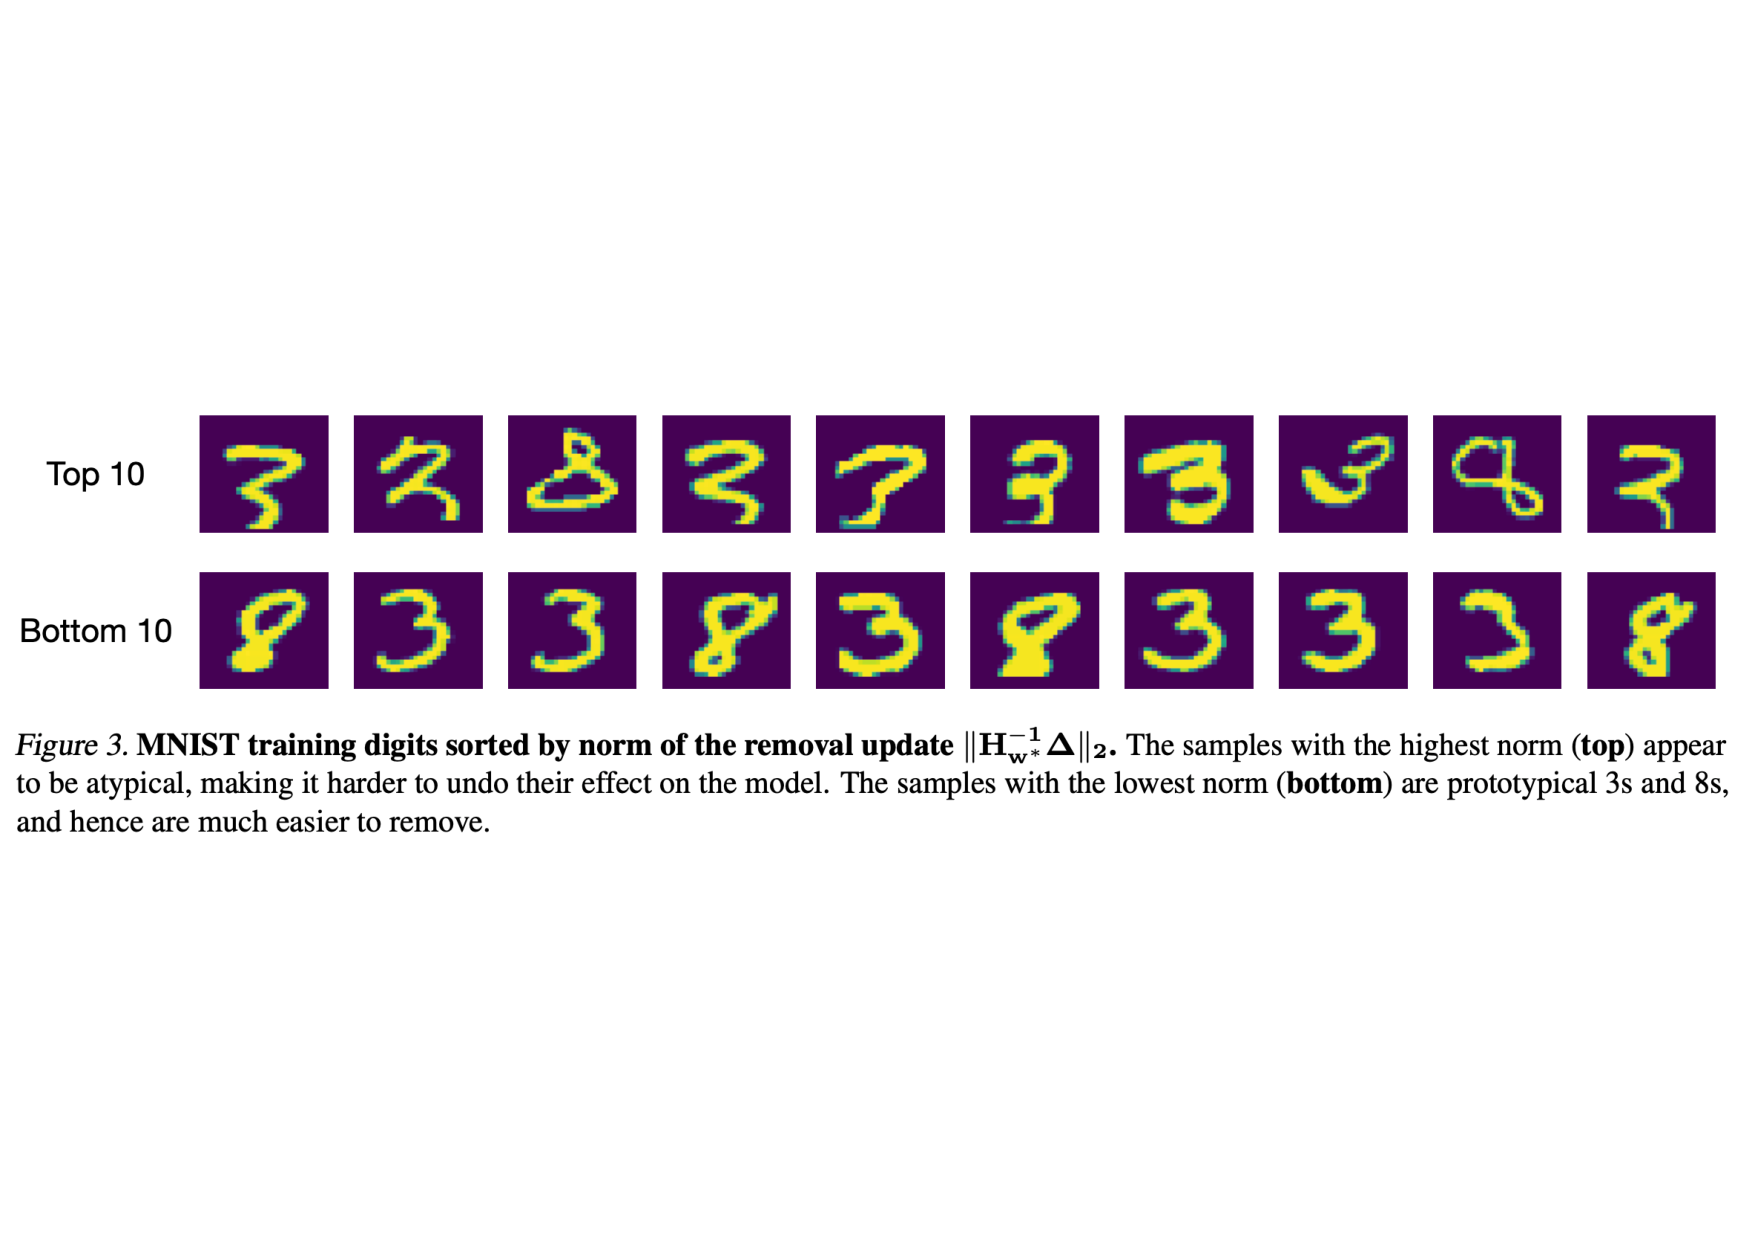
\includegraphics[width=\textwidth]{images/influence functions.pdf}
\end{frame}

\begin{frame}
  \frametitle{Certifing Removal}
  \begin{itemize}
    \item $\wminus$ is approximate close to minimizer of $\risk(\w;\datasetprime)$
    \item $\nabla\risk(\wminus;\datasetprime)$ is gradient residual and if non-zero, reveals Information
    \item Even a small $\|\nabla\risk(\wminus;\datasetprime)\|_{2}$ doesn't guarantee certifiable removal 
    \item Therefore, perturb loss at training time 
    \[
      \risk_{b}(\w;\dataset) = \sum_{i=1}^{n}\loss(\w^{T}\x_{i},y_{i})+\frac{\lambda n}{2}\|\w\|_{2}^{2} + \textbf{b}^{T}\w
    \]
    Where $\textbf{b}\in \mathbb{R}^{d}$ drawn randomly from some distribution
  \end{itemize}

\end{frame}

\begin{frame}
  \frametitle{Benefits and Drawbacks}
  \begin{block}{Benefits}
    \begin{itemize}
      \item Provides formal guarantee of statistical indistinguishability
      \item Works well with Differentially Private trained networks
      \item Uses influence functions to approximate data removal
    \end{itemize}    
  \end{block}
  \begin{alertblock}{Limitations}
    \begin{itemize}
      \item Requires inverting a Hessian matrix
      \item Non-convex loss functions not supported 
      \item Adding noise during training hurts model performance
      \item Very strict notion of removal
    \end{itemize}
    
  \end{alertblock}
\end{frame}
\subsection{Optimization}
\begin{frame}
  \myNset[2]
  \smartart
\end{frame}

\begin{frame}
  \frametitle{
    DeltaGrad \cite{wuDeltaGradRapidRetraining2020}
    }
  \begin{itemize}
    \item $\mech$ targets the Gradient Descent (GD) algorithm
    \item Naive retraining $\alg(\datasetprime)$ recomputed gradients over all remaining points
    \[
        \wu_{t+1} \leftarrow \wu_{t} - \frac{\eta_{t}}{n-r}\sum_{i\in \datasetprime}\nabla \risk_{i}(\wu_{t})
    \]
    \item Instead rewrite it as a \textit{leave-r-out} formula
    \[
      \wi_{t+1} = \wi_{t} - \frac{\eta_{t}}{n-r}\left[\sum_{i\in \dataset}\nabla \risk_{i}(\wi_{t}) -\sum_{i\in \removed} \nabla \risk_{i}(\wi_{t})\right]
    \]
    \item Much cheaper to compute $r$ gradients, when $r \ll n$
  \end{itemize}

\end{frame}

\begin{frame}
  \frametitle{Approximating $\sum_{i\in \dataset}\nabla \risk_{i}(\wi_{t})$}
  \begin{itemize}
    \item Need to use historical $\nabla \risk(\w_{t})$ to approximate $\nabla\risk(\wi_{t})$
    \item Taylor expansion around $\wi_{t}$ gives the following
    \[
       \nabla \risk(\wi_{t}) = \nabla \risk(\w_{t}) + \h_{t}\cdot(\wi_{t}-\w_{t}) 
    \]
    Where $\h_{t} = \int_{0}^{1}\h(\w_{t}+x(\wi_{t}-\w))dx$
    \item Maintaining a Hessian matrix is expensive, so leverage the L-BFGS algorithm to compute a Hessian-vector product
    \item This leads to issues in error bounds of the approximation
  \end{itemize}
    
\end{frame}

\begin{frame}
  \frametitle{Problem with Error Bound}
  \includegraphics[page=43,clip,trim=0.5cm 1cm 0cm 1cm,width=\textwidth]{images/Slides.pdf}
\end{frame}

\begin{frame}
  \frametitle{Controlling the Errors}
  \begin{itemize}
    \item Do explicit evaluations for $j_{0}$ "burn-in" iterations and then periodically every $T_{0}$ iterations
    \includegraphics[page=46,clip,trim=0.5cm 1cm 0cm 1cm,width=0.8\textwidth]{images/Slides.pdf}
  \end{itemize}
\end{frame}

\begin{frame}
  \frametitle{Benefits and Limitations}
  \begin{block}{Benefits}
    \begin{itemize}
      \item Handles both additions nad deletions of datapoints
      \item Can be applied to any ML model trained using Stochastic Gradient Descent
      \item Approximation guarantees and empirical results on 
    \end{itemize}
  \end{block}
  \begin{alertblock}{Limitaitons}
    \begin{itemize}
      \item Needs to cache all weights $\w_{t}$ and gradients $\nabla \risk(\w_{t})$ during training
      \item Requires tuning of $T_{0}$ and $j_{0}$ based on dataset
      \item For SGD, only works with large batch sizes ($>10000$), which hurts model performance 
    \end{itemize}
  \end{alertblock}
  

\end{frame}

\subsection{Information Theory}
\begin{frame}
  \myNset[3]
  \smartart
\end{frame}

\begin{frame}
  \frametitle{
    Eternal Sunshine of the Spotless Net \cite{golatkarEternalSunshineSpotless2020}
    }
  \begin{itemize}
    \item $P(\w | \dataset)$ distribution of algorithm $\alg$
    \item $\mech$ is called \emph{scrubbing function} applied to $\w$
    \item $P(M(\w)|\dataset)$ is distribution of possible weights after scrubbing
    \item Motivation: disallow attacker to use \textit{read-out function} $f(\w)$ to gain information about $\removed$
    \item Therefore, optimal scrubbing function must have 
    \[
      \KL(P(f(\mech(\w))|\dataset)~\|~P(f(S_{0}(\w))|\datasetprime))=0
    \]
    Where $S_{0}$ is a \textit{certificate} of forgetting
    \item To be agnostic of $f(\cdot)$, minimize
    \[
      \KL(P(\mech(\w)|\dataset)~\|~P(S_{0}(\w)|\datasetprime)) 
    \]
  \end{itemize}
\end{frame}

\begin{frame}
  \frametitle{Forgetting Lagrangian}
  \begin{itemize}
    \item A trivial noise scrubbing is $M(\w)=S_{0}(\w) = w+\sigma n$, where $n \sim \mathcal{N}(0,I)$
    \item As $\sigma \rightarrow \infty$, $\KL(p\|q)\rightarrow 0$, which invalidates the model 
    \item Define the \emph{Forgetting Lagrangian}:
    \[
      \mathcal{L} = \mathbb{E}_{\mech(\w)}[\risk_{\datasetprime}(\w)] + \lambda\KL(P(\mech(\w)|\dataset)~\|~P(S_{0}(\w)|\datasetprime)) 
    \]
    \item Use quadratic approximation and noise to scrub weights
    \item $\mech(\w) = h(\w)+n$ and $S_{0}=w + n^{\prime}$ where $h(\w)$ is deterministic and $n,n^{\prime} \sim \mathcal{N}(,\Sigma)$
  \end{itemize}

\end{frame}

\begin{frame}
  \frametitle{Scrubbing Example }
  \begin{center}
  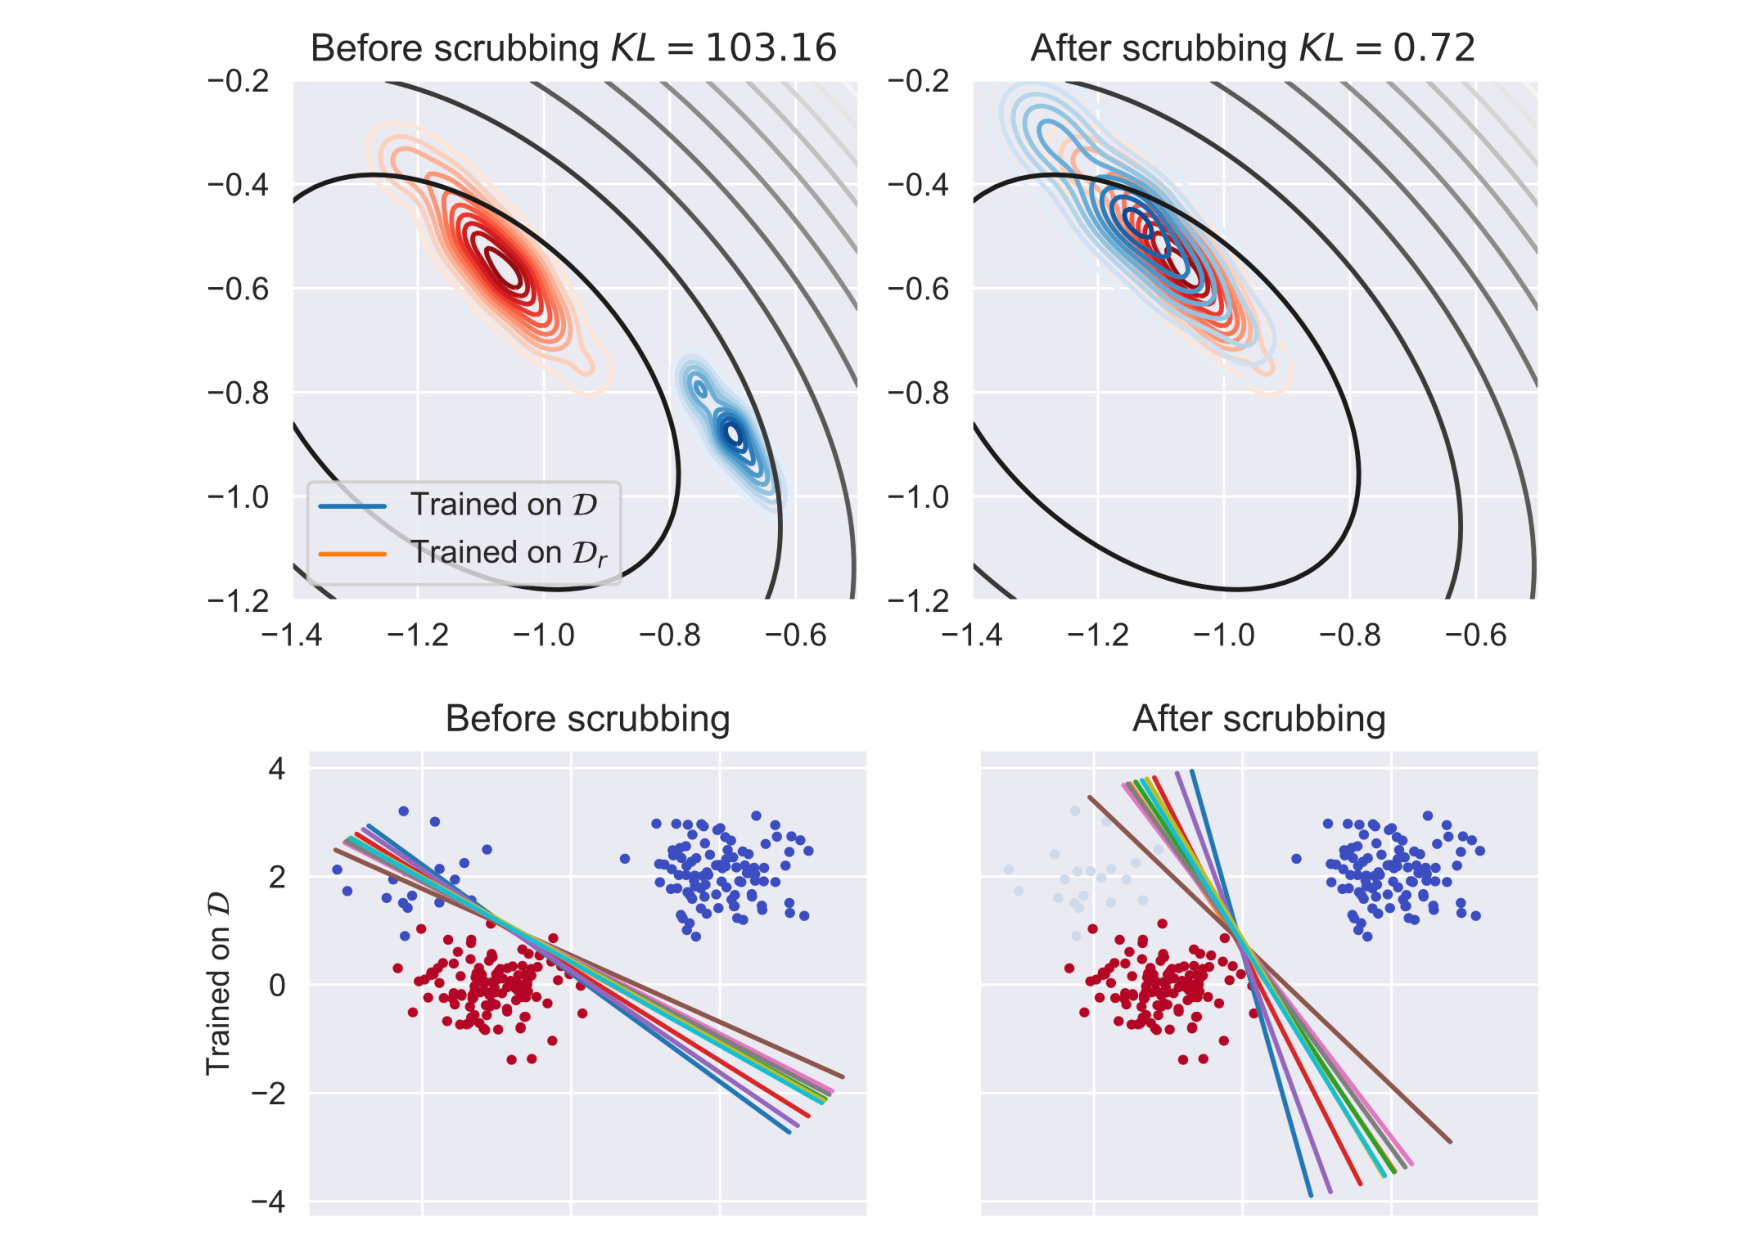
\includegraphics[width=0.9\textwidth]{images/scrubbing.pdf}
  \end{center}

\end{frame}
\begin{frame}
  \frametitle{Robust Quadratic Scrubbing}
  \begin{itemize}
    \item Noisy Newton update, as $t\rightarrow\infty$ is defined as 
    \[
      \mech_{t}(\w) = \w - \h^{-1}\nabla\risk_{\datasetprime}(\w) + (\lambda\sigma^{2}_{h})^{1/4}\h^{-1/4}
    \]
    Where $\h = \nabla^{2}(\risk_{\datasetprime}(\w))$, $\sigma_{h}$ represents error in approximating SGD with a continuous gradient flow and $\lambda$ hyperparameter
    \item For Deep Neural Networks, Hessian matrix is expensive to compute and store
    \item Simplified scrubbing to only adding noise 
    \[
      \mech(\w) = \w + (\lambda\sigma^{2}_{h})^{1/4}F^{-1/4}
    \]
    \item $F$ is the Fisher Information Matrix, computed using the Levenberg- Marquardt semi-positive-definite approximation of $\nabla^{2}\risk_{\dataset}(\w)$
  \end{itemize}
  
\end{frame}
\begin{frame}
  \frametitle{Benefits and Limitations}
  \begin{block}{Benefits}
    \begin{itemize}
      \item Works for Deep Neural Networks
      \item Allows to remove a entire class, multiple classes, or a subset of a class of the training dataset
      \item Process is optimal if quadratic assumptions hold true
    \end{itemize}
  \end{block}

  \begin{alertblock}{Limitations}
    \begin{itemize}
      \item Space and time complexity of approach unknown
      \item Considers worst case of attacker using any read-out function $f(\cdot)$
      \item Results based on stability of SGD after pre-training networks
    \end{itemize}
  \end{alertblock}
\end{frame}

\subsection{Novel Pipelines}
\begin{frame}
  \myNset[4]
  \smartart
\end{frame}


\begin{frame}
  \frametitle{
    Machine Unlearning: SISA \cite{bourtouleMachineUnlearning2020}
    }
  SISA Framework 
  \begin{itemize}
    \item {\bf Sharded}:\\
    Dataset is divided into $S$ disjoint shards, $\cap_{k \in [S]}\dataset_{k}=\emptyset$ and $\cup_{k\in[S]}\dataset_{k}=\dataset$
    \item {\bf Isolated}:\\
    ML models are trained on each data shard $\dataset_{k}$ in isolation to other data shards
    \item {\bf Sliced}:\\
    Further, each shard $\dataset_{k}$ is sliced into $R$ disjoint slices. Incrementally present shards during training
    \item {\bf Aggregated}:\\
    During inference aggregate predictions from individual models 
  \end{itemize}
\end{frame}

\begin{frame}
  \frametitle{SISA Framework}
  \begin{center}
    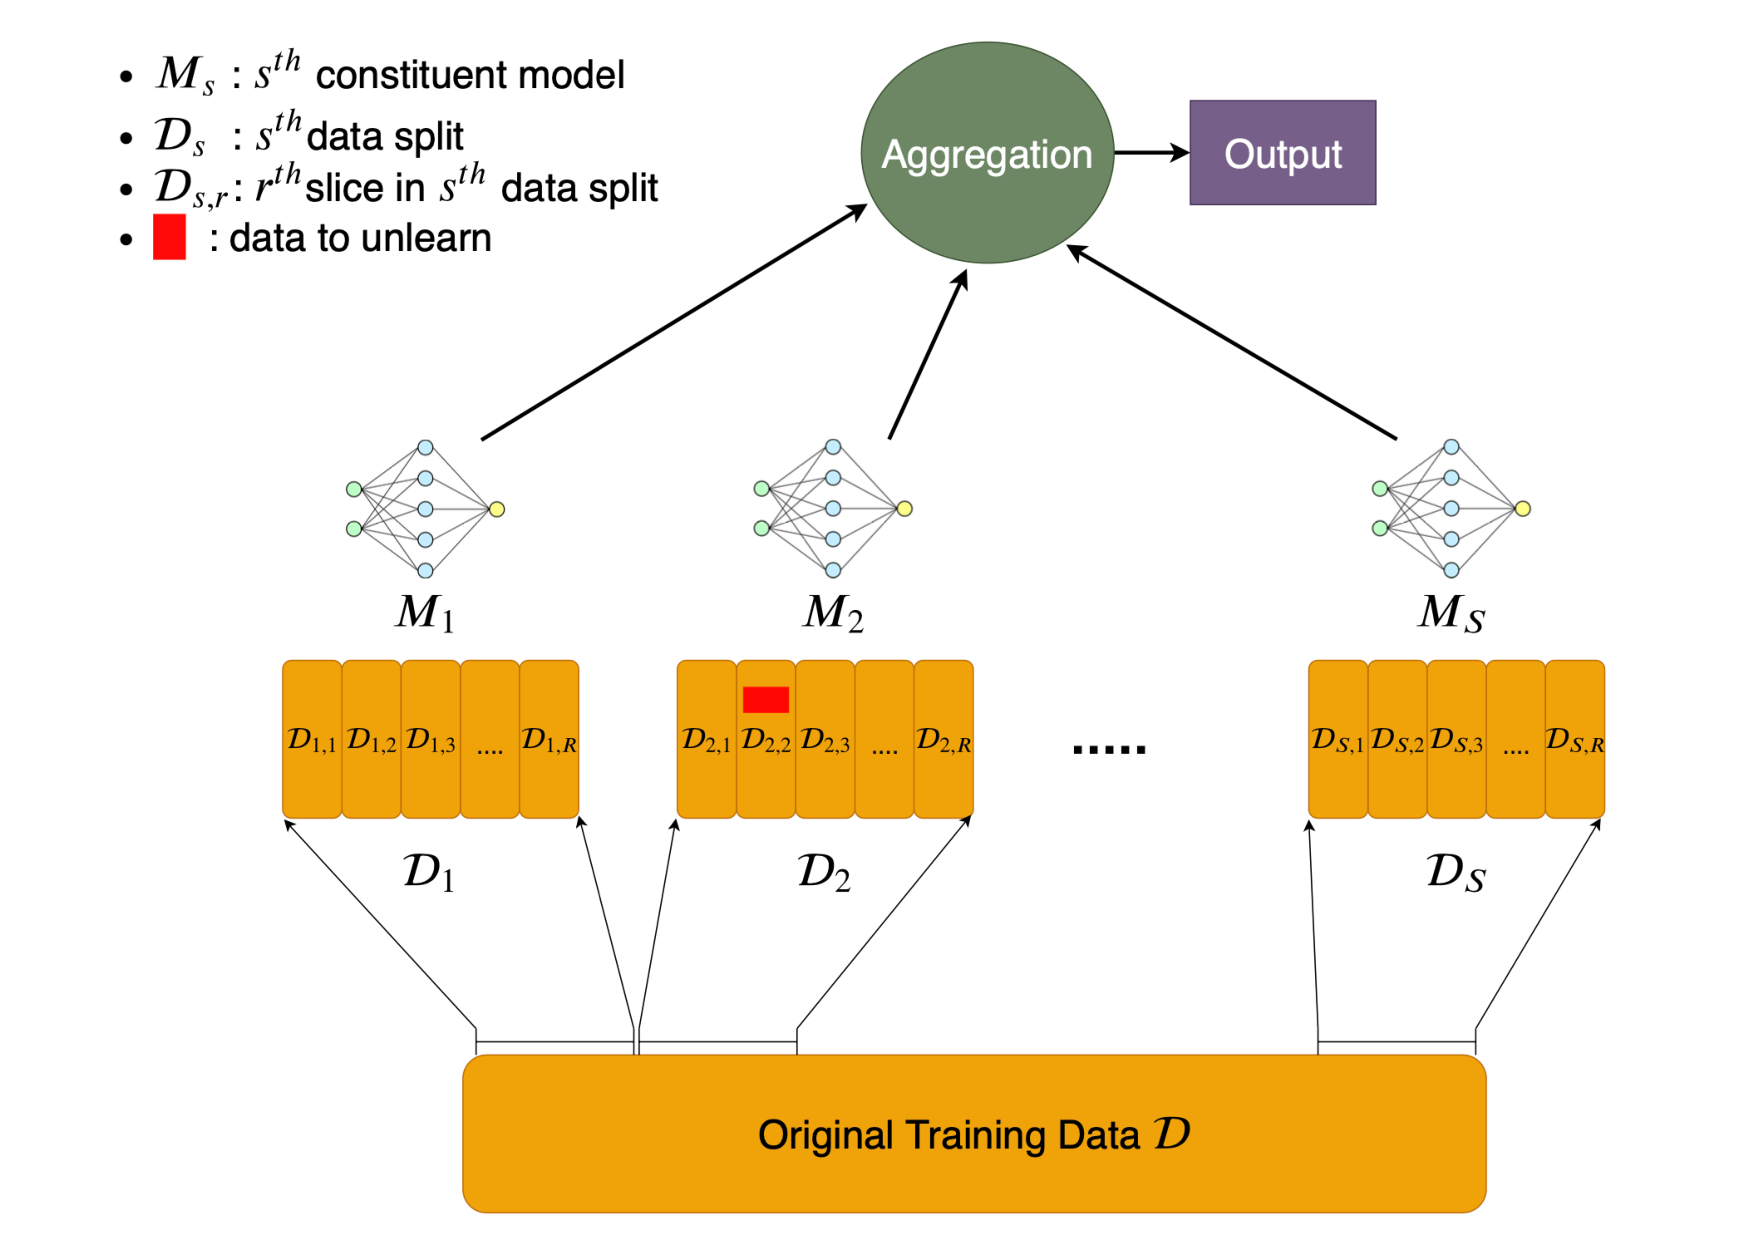
\includegraphics[width=0.9\textwidth]{images/SISA.pdf}
  \end{center}
\end{frame}

\begin{frame}
  \frametitle{Benefits and Drawbacks}
  \begin{block}{Benefits}
    \begin{itemize}
      \item Service providers have \textit{plausible removal} of data
      \item Practical approach reduces the overhead of unlearning
      \item Can utilize distributional of remove requests for sharding
    \end{itemize}
  \end{block}
  \begin{alertblock}{Drawbacks}
    \begin{itemize}
      \item Training of isolated shards might lead to weak learners for especially complex tasks
      \item Sharding and slicing increase the overall space complexity of the approach
      \item Distribution aware sharding might lead to biased models 
    \end{itemize}      
  \end{alertblock}
\end{frame}

\section{Next Directions}
\begin{frame}
  \frametitle{Ideas}
  \begin{itemize}
    \item Analytical and empirical comparison of various approaches
    \item Investigate \textit{influence functions} for deep networks \cite{kohUnderstandingBlackboxPredictions2017,basuInfluenceFunctionsDeep2020}
    \item Research SGD convergence and non-convex loss properties \cite{liConvergenceAnalysisTwolayer2017a,liVisualizingLossLandscape2018}
    \item Implement SGD as Adaptive Statistical Query (ASQ) learning \cite{caoMakingSystemsForget2015} and perform unlearning
  \end{itemize}

  

\end{frame}

\begin{frame}[allowframebreaks]
  \frametitle{References}
  \bibliography{UpdateMl}
  \bibliographystyle{apalike}
\end{frame}



\end{document}  